% Credit: Хабибулин Артур 0301 СПбГЭТУ "ЛЭТИ" 2024
\documentclass[14pt, a4paper]{extarticle}

% Включаем файлы с настройками
% Поддержка Русского языка
\usepackage{polyglossia}

% Для 14го размера текста
\usepackage{extsizes}

% Для полуторного интервала
\usepackage{setspace}

% Для вставки pdf файлов
\usepackage{pdfpages}

% Настройка подписей
\usepackage{caption}

% Математические символы и специальные environments для лемм и прочего
\usepackage{amsmath}
\usepackage{amssymb}
\usepackage{mathtools}

% Ссылки и гиперссылки
\usepackage[unicode]{hyperref}

% Отступ слева 1.25см
\usepackage{indentfirst}

% Для настройки списков
\usepackage{enumitem}

% Вставка картинок
\usepackage{graphicx}
% Для опции "H" картинки, чтобы она вставала там же, где указана в сыром тексте
\usepackage{float}

% Форматирование заголовков
\usepackage{titlesec}

% Библиография 
% \usepackage[citestyle=numeric-comp, sorting=none, style=ieee, backend=biber]{biblatex}

% Библиография по ГОСТ 2008
\usepackage[style=gost-numeric, backend=biber, language=auto, autolang=other, sorting=none]{biblatex}

% Таблица с выравниванием по ширине
\usepackage{tabularx}
% Длинные таблицы, которые не помещаются на одну страницу
\usepackage{longtable}

% Разбиение ячеек и столбцов на несколько строк или колонок
\usepackage{multirow}
\usepackage{multicol}

% Оформление листингов
\usepackage[newfloat]{minted}
\usepackage{listings}
\usepackage{lstfiracode}
\usepackage{color}

% Настройка стиля ToC
\usepackage{tocloft}

% Улучшенное форматирование pdf 
\usepackage{microtype}

% Установка языков документа
\setdefaultlanguage[spelling=modern]{russian}
\setotherlanguage{english}

% Установка TNR для различных стилей текста
\defaultfontfeatures{Mapping=tex-text}
\setmonofont{Times New Roman}
\setromanfont{Times New Roman}
\setmainfont{Times New Roman}
\newfontfamily\cyrillicfont{Times New Roman}

\urlstyle{same}

% Полуторный интервал
\onehalfspacing

% Красная строка
\setlength{\parindent}{1.25cm}

% Подсветка ссылок
\hypersetup{
    colorlinks=false,
    urlcolor=blue,
    filecolor=blue,
    citecolor=green,
    urlcolor=blue
}

% Папка с изображениями
\graphicspath{{./img/}}
% Длина изображений по умолчанию
\setkeys{Gin}{width=16cm}

% Форматирование подписей к картинками, листингам, таблицам
\captionsetup[figure]{name={Рисунок}, labelsep = endash, font = small, justification=centering}
\captionsetup[table]{name={Таблица}, labelsep = endash, font = small, justification=raggedleft, singlelinecheck=false, position = top}
\captionsetup[listing]{name={Листинг}, labelsep = colon, font = small, justification=raggedright, singlelinecheck=false, position = top}

% Форматирование заголовков глав и подглав
\titleformat
	{\section}
	[hang]
	{\normalfont\bfseries\center}
	{\arabic{section}. }
	{1ex}
	{\MakeUppercase}
\titlespacing
	{\section}
	{\parindent}
	{5ex}
	{4ex}
\titleformat
	{\subsection}
	[hang]
	{\normalfont\bfseries}
	{\arabic{section}.\arabic{subsection}. }
	{1ex}
	{}
\titlespacing
	{\subsection}
	{\parindent}
	{4ex}
	{4ex}

% Нумерация рисунков и таблиц включает номер главы
\counterwithin{figure}{section}
\counterwithin{table}{section}
% Можно включить и для формул
%\counterwithin{equation}{section}

% Установка шрифта для листингов minted
\setmonofont{FiraCode-Regular.ttf}[
	SizeFeatures={Size=10},
	Path = setup/,
	Contextuals=Alternate
]

% Настройка подсветки кода 
\usemintedstyle{gruvbox-light} % делает подсветку для кода

% Убираем жирный шрифт из названия ToC (Table of content)
\renewcommand*\cfttoctitlefont{\normalfont\bfseries\MakeUppercase}
% Убираем жирный шрифт из записей в ToC
\renewcommand{\cftsecfont}{}
% Убираем жирный шрифт из номеров страниц в ToC
\renewcommand{\cftsecpagefont}{}

% Уменьшаем расстояние между элементами списка 
\setlist[enumerate]{itemsep=1.0pt}

% Минимизируем количество переносов
\tolerance = 500
\hyphenpenalty = 20000
\emergencystretch = 1cm
% Вставка изображения \image{}{}[][]

% Обязательные аргументы:
% 	1. Название изображения в папке img без расширения
% 	2. Подпись к рисунку

% Опциональные аргументы:
% 	1. Размер картинки. По умолчанию: 16cm
% 	2. label для ссылок
\NewDocumentCommand\image{mmoo}{
    \begin{figure}[H]
        \centering
        \includegraphics[width=#3, keepaspectratio]{#1}
        \caption{#2}
        \label{#4}
    \end{figure}
}

% Заголовок для лабораторной работы \sectionlab{}
% Отличается от стандартного  измененным стилем и отсутствием нумерации
%
% Обязательные аргументы:
% 	1. Текст заголовка
\NewDocumentCommand\sectionlab{m}{
    \titleformat
	{\section}
	[hang]
	{\normalfont\bfseries\filouter}
	{}
	{0pt}
	{}
\titlespacing
	{\section}
	{\parindent}
	{5ex}
	{4ex}

    \section{#1}

    \titleformat
	{\section}
	[hang]
	{\normalfont\bfseries\center}
	{\arabic{section}. }
	{1ex}
	{\MakeUppercase}
\titlespacing
	{\section}
	{\parindent}
	{5ex}
	{4ex}
}

% Вставка заголовка приложения \sectionappendix[]
% Автоматически нумерует приложения по латинским буквам. Позволяет получать полное название приложения с гиперссылкой через \nameref

% Опциональные аргументы:
% 	1. label для ссылок 
\makeatletter
\NewDocumentCommand\sectionappendix{o}{
    \newpage
    \refstepcounter{section}
    \stepcounter{appendix_counter}
    \section*{Приложение \Alph{appendix_counter}}
    \addcontentsline{toc}{section}{\protect\numberline{}Приложение \Alph{appendix_counter}}
    \edef\@currentlabelname{Приложение \Alph{appendix_counter}}
    \phantomsection
    \label{#1}
}
\makeatother

% Макрос для ссылки на Рисунок в форме "Рисунок 1" \picref{}

% Обязательный аргументы:
% 	1. label картинки, на которую ссылка
\NewDocumentCommand{\picref}{m}{
    \hyperref[{#1}]{Рисунок~\ref*{#1}}
}

% Макрос для ссылки на Листинг в форме "Листинг 1" \lstref{}

% Обязательный аргументы:
% 	1. label картинки, на которую ссылка
\NewDocumentCommand{\lstref}{m}{
    \hyperref[{#1}]{Листинг~\ref*{#1}}
}

% Макрос для ссылки на Таблицу в форме "Таблица 1" \tblref{}

% Обязательный аргументы:
% 	1. label картинки, на которую ссылка
\NewDocumentCommand{\tblref}{m}{
    \hyperref[{#1}]{Таблица~\ref*{#1}}
}


\usepackage{listings} % библиотека листингов
\usepackage{color} % подсветка листинга

\definecolor{mygreen}{rgb}{0,0.6,0}
\definecolor{mymauve}{rgb}{0.58,0,0.82}

\lstset{ % Подробнее про настройку листингов https://en.wikibooks.org/wiki/LaTeX/Source_Code_Listings
  backgroundcolor=\color{white},        % цвет фона
  basicstyle=\ttfamily\small,    % семейсто, размер шрифта
  breakatwhitespace=true,               % разрыв строк только при пробеле
  breaklines=true,                      % перенос строк
  captionpos=t,                         % месторасположение подписи bottom
  commentstyle=\color{mygreen},         % цвет комментария (не распростроняется на кириллицу)
  keepspaces=true,                      %
  keywordstyle=\color{blue},            %
  showspaces=false,                     % отключена замена пробелов на нижние подчеркивания
  showstringspaces=false,               % отключена замена пробелов на нижние подчеркивания
  showtabs=false,                       % отключена замена табуляций на нижние подчеркивания
  stepnumber=1,                         %
  stringstyle=\color{mymauve},          % цвет литералов
  tabsize=4,                            %
}

% Подписи к листингам на русском языке.
\renewcommand\lstlistingname{Листинг}
\renewcommand\lstlistlistingname{Листинги}

% Намеренно не в файле packages
\usepackage[top=2cm, bottom=2cm, left=3cm, right=1cm]{geometry}

% Счетчик приложений
\newcounter{appendix_counter} 

% Метаданные для pdf
\author{Автор Авторович}
\title{VKR_or_lab}
\date{Сегодня 2024}

% Подключения файла с библиографией
\addbibresource{refs.bib}

% Начало документа
\begin{document}

% Структура ВКР
% По порядку: титульный лист, аннотация(реферат), содержание работы, введение, главы, заключение, список источников, приложения
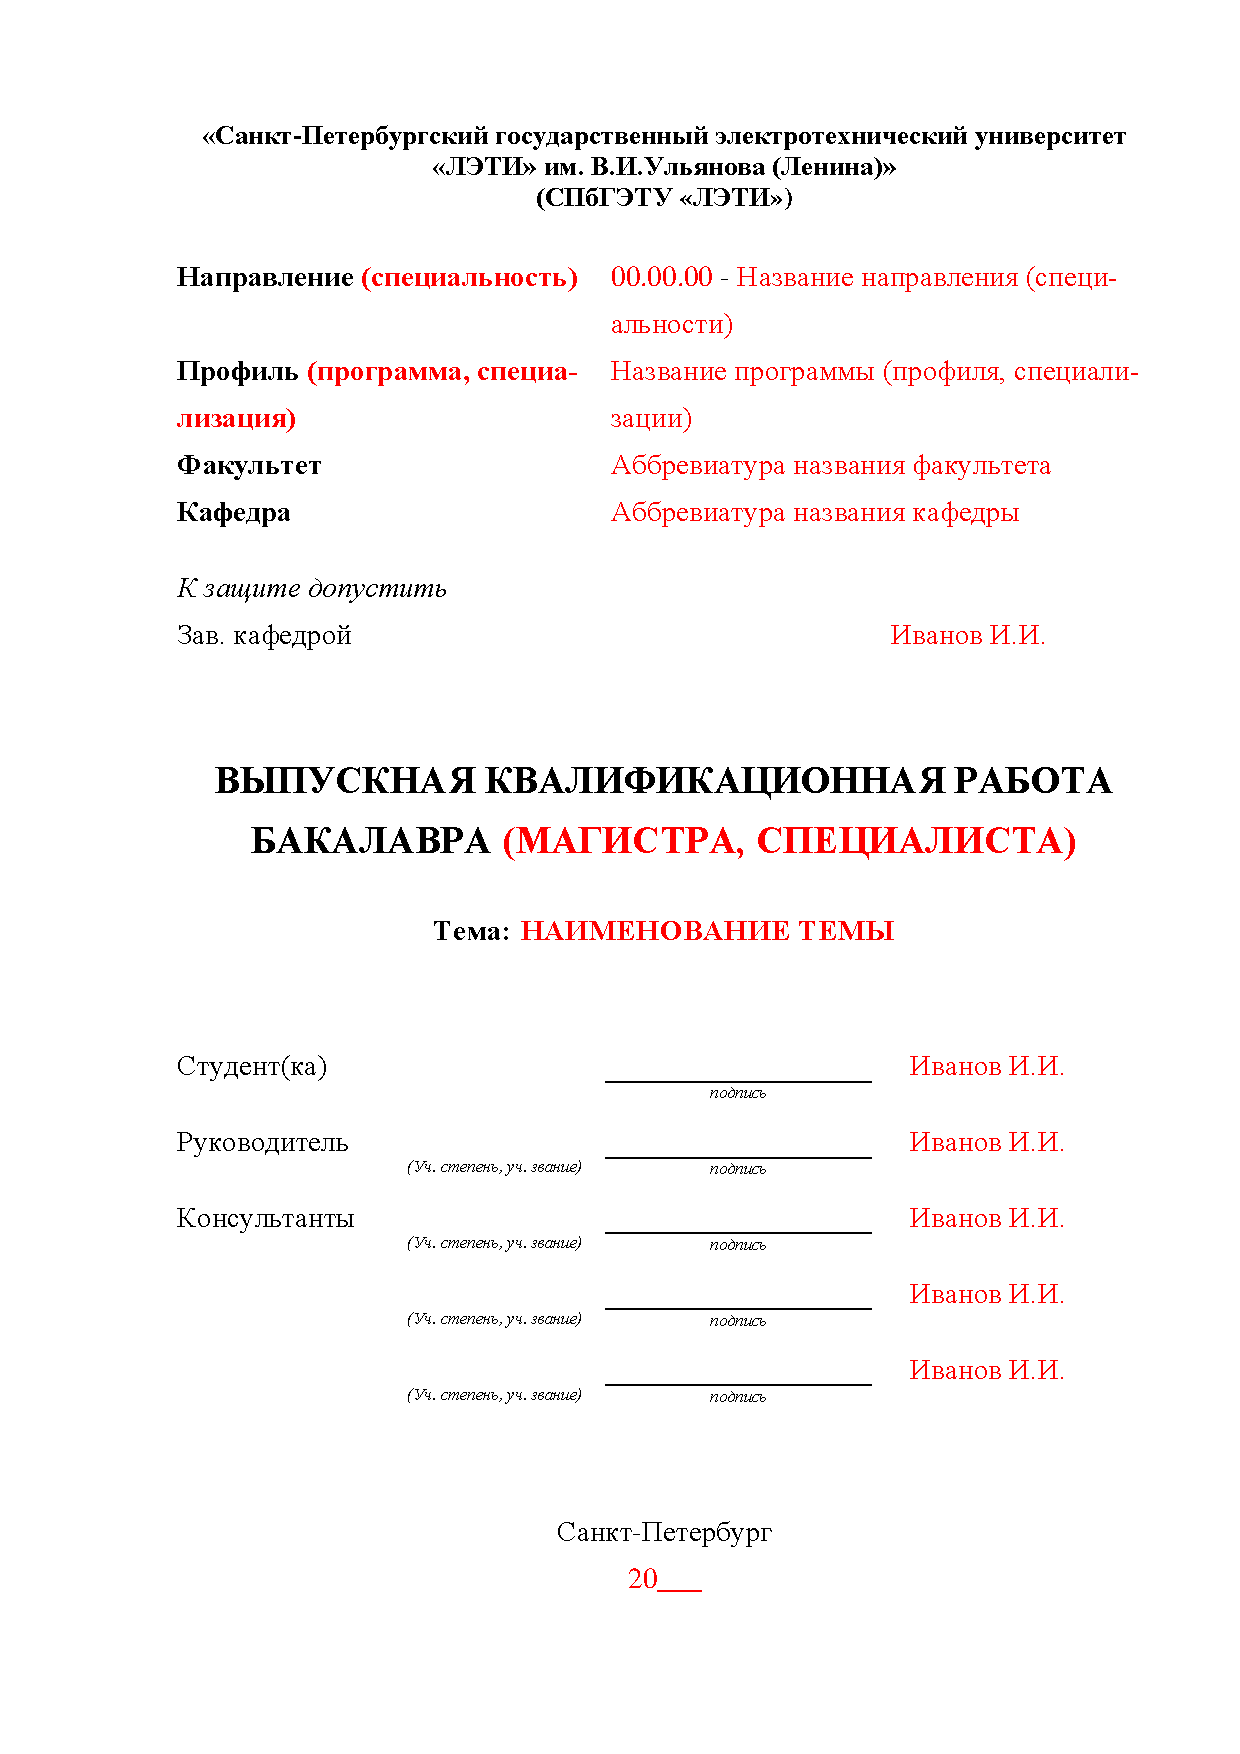
\includepdf[pages={1-}]{title/vkr_title.pdf}
\newpage
\section*{Реферат}

Пояснительная записка 00 стр., 00 рис., 0 табл.,  00 ист., 00 прил.

\MakeUppercase{тег, тег, тег, тег}

Текст аннотации кратко отражающий суть работы


\newpage
\section*{Abstract}

Brief Abstract that describes the paper


\newpage
\newpage
\renewcommand*\contentsname{Содержание}
\begin{center}
    \tableofcontents
\end{center}
\newpage
\newpage
\section*{Введение}
\addcontentsline{toc}{section}{\protect\numberline{}Введение}

Введение к работе

\newpage
\section{Первая глава}

\subsection{Первая подглава первой главы}
Далее будут описаны примеры использования основных команд шаблона.

Вставка картинки (\picref{pic:example1}) и ссылка на нее:

\image{example_img}{Подпись к картинке}[8cm][pic:example1]

Вставка формулы \eqref{eq:example1} и ссылка на нее:

\begin{equation}
    \label{eq:example1}
    \frac{\delta f}{\delta t} = \lim_{h \rightarrow 0} \left[ \frac{f (t + h) - f(t)}{h} \right]
\end{equation}

Вставка таблицы(\tblref{tbl:example1}) и ссылки на нее:

\begin{table}[H]
    \centering
    \caption{Пример таблицы}
    \label{tbl:example1}
    \begin{tabular}{| c | c | c |}
        \hline
        row & row & row \\
        \hline
        row & row & row \\
        \hline
        row & row & row \\
        \hline
        row & row & row \\
        \hline
        row & row & row \\
        \hline
    \end{tabular}
\end{table}

Листинг minted (\lstref{code:example1}) и ссылка на него:

\begin{listing}[H]
    \caption{Пример листинга}
    \label{code:example1}
    \inputminted[breaklines=true, framesep=10pt, fontsize=\footnotesize, firstline=1, lastline=8]{python}{listing/code_sample.py}
\end{listing}

Листинг listings (\lstref{code:example2}) и ссылка на него:

\begin{listing}[H]
    \caption{Пример листинга}
    \label{code:example2}
    \lstinputlisting[language=Python, firstline=1, lastline=8]{listing/code_sample.py}
\end{listing}

Ссылка на приложение (\nameref{appendix:calc})

Пример цитаты \cite{domanovdi}

Пример нескольких цитат \cite{domanovdi,duportail:alu,fsrf40}

\subsection{Вторая подглава первой главы}

\subsection{Третья подглава первой главы}
\section{Вторая глава}
\subsection{Первая подглава второй главы}

\subsection{Вторая подглава второй главы}
\subsection{Третья подглава второй главы}
\section{Третья глава}
\subsection{Первая подглава третьей главы}
\subsection{Вторая подглава третьей главы}
\subsection{Третья подглава третьей главы}
\section{Экономическое обоснование шаблона ВКР}
\newpage
\section*{Заключение}
\addcontentsline{toc}{section}{\protect\numberline{}Заключение}

Заключительные слова

\newpage
\newpage
\renewcommand*\refname{Список использованных источников}
\nocite{*}
\printbibliography
\addcontentsline{toc}{section}{\protect\numberline{}Список использованных источников}
\sectionappendix[appendix:calc]
\inputminted[breaklines=true, framesep=10pt, fontsize=\footnotesize, firstline=1]{python}{listing/code_sample.py}


\sectionappendix[appendix:bigtable]
\begin{longtable}{ 
    | m{10em}
    | m{10em} 
    | m{10em} | }
    
    \hline
    data & data & data\\
    \hline
    row & row & row\\
    \hline   
    row & row & row\\
    \hline   
    row & row & row\\
    \hline   
    row & row & row\\
    \hline   
    row & row & row\\
    \hline   
    row & row & row\\
    \hline   
    row & row & row\\
    \hline   
    row & row & row\\
    \hline   
    row & row & row\\
    \hline   
    row & row & row\\
    \hline   
    row & row & row\\
    \hline   
    row & row & row\\
    \hline   
    row & row & row\\
    \hline   
    row & row & row\\
    \hline   
    row & row & row\\
    \hline   
    row & row & row\\
    \hline   
    row & row & row\\
    \hline   
    row & row & row\\
    \hline   
    row & row & row\\
    \hline   
\end{longtable}

% Структура лабораторной работы
% 
% \pagenumbering{gobble}
\clearpage
\begin{center}	
	МИНОБРНАУКИ РОССИИ\\
	САНКТ-ПЕТЕРБУРГСКИЙ ГОСУДАРСТВЕННЫЙ\\
	ЭЛЕКТРОТЕХНИЧЕСКИЙ УНИВЕРСИТЕТ\\
	«ЛЭТИ» ИМ. В.И. УЛЬЯНОВА (ЛЕНИНА)\\
	Кафедра САПР

	\vspace{54mm}

	ОТЧЕТ\\
	по лабораторной работе №0 \\
	по дисциплине «Очень интересный предмет» \\
	Тема: Очень интересная тема

	\vspace{65mm}

	\def\arraystretch{1.5}
	\begin{tabularx}{\textwidth}{ >{\hsize=7cm}X >{\hsize=4cm}X  >{\centering\arraybackslash}X }
		Студент гр. 0000 & & Студент А.Б. \\ \cline{2-2}
		%Студент гр. 0000 & & Студент В.Г. \\ \cline{2-2}
		%Студент гр. 0000 & & Студент Д.Е. \\ \cline{2-2}
		Преподаватель & & Преподаватель А.Б. \\ \cline{2-2}
	\end{tabularx}
	\def\arraystretch{1}

	\vfill
	Санкт-Петербург\\
	2024
\end{center}
\newpage
\pagenumbering{arabic}
\setcounter{page}{2}
% \sectionlab{Цель работы}

Цель работы, которая обязательно будет достигнута

\sectionlab{Содержание работы}

Какой-то текст, какие-то наблюдения, может даже картинки с подписями.

\sectionlab{Выводы}

Благодаря картинками с подписями цель работы точно была достигнута

\end{document}